\chapter{Evaluation and Discussion}
\label{chap:evaluation-and-discussion}

\section{Evaluation Metrics}

As NIR colorization has two main application contexts: providing human users more interpretable images and to improve object recognition results by enriching the input with more information.
To assess the effectiveness of both models, we define qualitative evaluation categories and quantitative evaluation metrics based on their ability to achieve these goals.

\subsection{Quantitative Evaluation Metrics}
Due to the unpaired setting, in the quantitative evaluation classic solutions, such as the difference between the absolute intensity values or SSIM \parencite{ssim}, cannot be applied. Fortunately, methods for comparing the general image similarity of two sets, such as FID \parencite{ttur} or
comparing classification results using an off-the-shelf network, are well known to quantitatively assess the quality of image translation.

\subsubsection*{FID}
To measure how close the generated images are to the real images concerning human perception, the \textit{Fréchet Inception Distance} (FID) \parencite{ttur} is a commonly used metric.
It empirically estimates how the human eye perceives images for a set of images and computes the distance between two such set representations.
First, a pre-trained InceptionV3 model evaluates each image of the image set and the activation of the last layer is considered the "human perception approximation".
Then for all activation vectors of the evaluated images in the images set, a multidimensional Gaussian is fitted over those activation vectors.
This is done for two image sets, and later the two Gaussians are compared using the Fréchet distance \parencite{ttur}.
Intuitively, if the generated images are realistic, the statistics of features in a classification network should be similar to the real ones.

\todo{Add figure visualizing FID}

\label{sec:evaluate-fid}
\todo{Discuss usage of FID}

\subsection{Qualitative Evaluation Methods}
For qualitative evaluation, we define categories on how we determine the superior generated images. These are again based on the two main application contexts.

The first category describes the \textit{naturality} of an image, where the generated images should resemble how humans perceive the world, without artifacts or periodic patterns that can affect visual perception.

The second category refers to the \textit{content preservation} of the input image. This should help humans as well as object detection systems to find and classify animals accurately.

\textit{Hallucinations}, as artifacts or scene elements that are not in the input image, contradict naturality and content preservation, and therefore are undesirable.

\section{Unconditional Diffusion Model}
First we evaluate the unconditional sampling of the diffusion model and therefore validate \parencite{diffusion-beats-gans}'s results for image synthesis in still hold for this dataset:

\begin{table}[htp!]
    \centering
    \begin{tabular}{c | c}
        Model                   & FID  $\downarrow$ \\
        \hline\hline
        CycleGAN                & 98.10             \\
        Unconditional Diffusion & 95.73
    \end{tabular}
    \caption{
        \textbf{Quantitative Evaluation.} CycleGAN and the diffusion model trained on Snapshot Serengeti \parencite{serengeti} containing only night NIR and RGB images.
        Comparing the FID calculated between the test dataset and the generated images.
    }
    \label{fig:quantitative-evaluation-unconditional-sampling}
\end{table}

\begin{figure}[htp!]
    \centering
    \setkeys{Gin}{width=1\linewidth}
    \begin{tabularx}{\textwidth}{Y Y Y !{\space} Y Y Y}
        RGB                                                                                    & CycleGAN                                                                                         & Diffusion                                                                                    & RGB                                                                                    & CycleGAN                                                                                         & Diffusion                                                                                    \\
        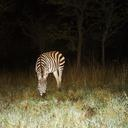
\includegraphics{gfx/unconditional-diffusion-sampling-qual/rgb_S2_B04_R3_IMAG0432.jpg} & \includegraphics{gfx/unconditional-diffusion-sampling-qual/cyclegan_S2_B06_R1_PICT0128_fake.png} & 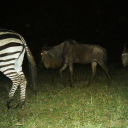
\includegraphics{gfx/unconditional-diffusion-sampling-qual/diffusion_S2_C07_R1_PICT0028.png} & 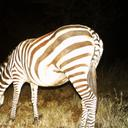
\includegraphics{gfx/unconditional-diffusion-sampling-qual/rgb_S2_B04_R3_IMAG0471.jpg} & 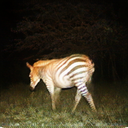
\includegraphics{gfx/unconditional-diffusion-sampling-qual/cyclegan_S2_B06_R1_PICT0279_fake.png} & 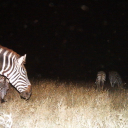
\includegraphics{gfx/unconditional-diffusion-sampling-qual/diffusion_S2_B07_R3_PICT0492.png} \\
        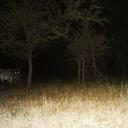
\includegraphics{gfx/unconditional-diffusion-sampling-qual/rgb_S2_B05_R1_IMAG0084.jpg} & \includegraphics{gfx/unconditional-diffusion-sampling-qual/cyclegan_S2_B06_R1_PICT0387_fake.png} & 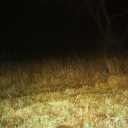
\includegraphics{gfx/unconditional-diffusion-sampling-qual/diffusion_S2_B06_R1_PICT0387.png} & 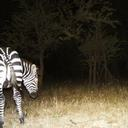
\includegraphics{gfx/unconditional-diffusion-sampling-qual/rgb_S2_B05_R1_IMAG0132.jpg} & \includegraphics{gfx/unconditional-diffusion-sampling-qual/cyclegan_S2_B06_R3_PICT1364_fake.png} & 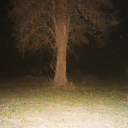
\includegraphics{gfx/unconditional-diffusion-sampling-qual/diffusion_S2_B08_R1_PICT0359.png} \\
        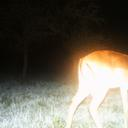
\includegraphics{gfx/unconditional-diffusion-sampling-qual/rgb_S2_B05_R2_IMAG0016.jpg} & 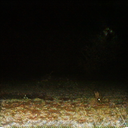
\includegraphics{gfx/unconditional-diffusion-sampling-qual/cyclegan_S2_B06_R3_PICT3848_fake.png} & 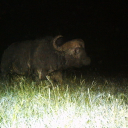
\includegraphics{gfx/unconditional-diffusion-sampling-qual/diffusion_S2_B07_R2_PICT0277.png} & 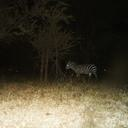
\includegraphics{gfx/unconditional-diffusion-sampling-qual/rgb_S2_B05_R3_IMAG1018.jpg} & 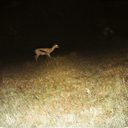
\includegraphics{gfx/unconditional-diffusion-sampling-qual/cyclegan_S2_B07_R1_PICT3274_fake.png} & 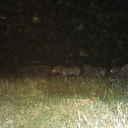
\includegraphics{gfx/unconditional-diffusion-sampling-qual/diffusion_S2_B07_R1_PICT3274.png}
    \end{tabularx}
    \caption{
        \textbf{Qualitative Evaluation.} Left to right: Sample image from the RGB domain of the Serengeti test dataset \parencite{serengeti},
        sample produced by CycleGAN \parencite{mehri} and an unconditional sample produced by the diffusion model \parencite{diffusion-beats-gans}.
    }
    \label{fig:qualitative-evaluation-unconditional-sampling}
\end{figure}

Qualitatively we observe in \autoref{fig:qualitative-evaluation-unconditional-sampling} that the diffusion model is capable to create realistic images.
As in the training dataset, many images without animal present are produced.
Images containing animals illustrates the model performs exceptionally well in creating realistic ones with matching lighting.
Only in few cases, trees are generated with undistinguishable branches. This is the only flaw which can be observed.

Quantitatively in \autoref{fig:quantitative-evaluation-unconditional-sampling} we see, the diffusion network only slightly outperforms CycleGAN's performance.
We expect clearer distinction to CycleGAN when a larger U-Net would be used, more training iterations and a larger dataset would be used.
Compared to \textcite{diffusion-beats-gans} we had to do trade-offs due to a lack of ultra-high performant computational resources.
Nevertheless, it can be argued that this unconditional diffusion model is capable enough to be a basis for a good colorization.

\todo{Provide hyperparameter}

\section{Loss-Guided and Correction-Guided Sampling}
As introduced in \autoref{sec:conditional-sampling} we suggest a differentiation into
\textit{loss-guided} (\autoref{sec:energy-guided-sampling}) and \textit{correction-guided} (\autoref{sec:correction-guided-sampling}) sampling.

At first sight we observe greater simplicity in defining a loss or energy rather than correcting an image.
Generally when using the correction-guided approach, the current sampled image has to be decomposed into multiple parts,
one part being the one to be modified and the second one being the remainder.
As the decomposition function must be invertible to create a functional framework, not all problems or properties are suited to be modelled like this.
Formulation as an energy is often easier to obtain and sometimes the only possibility.

In the case of near-infrared colorization both methods are implementable.
We evaluate for the context of near-infrared colorization which method should be used.
For both cases we condition using near-infrared images by assuming the intensity of the sample should be equal to the near-infrared image.
We discuss this particular conditioning method separately in \autoref{sec:nir-as-intensity-approximation-evaluation}.
In \autoref{fig:qualitative-evaluation-loss-guided-vs-correction-guided} we demonstrate the difference when formulating exactly the same property as energy-guided sampling and as correction-guided sampling.
It can be observed that the contours appear generally more noisy in the loss-guided sampling.
This observation is also quantitatively reflected, the FID of the loss-guided sampling is $23.64$ points higher than of the correction-guided approach (\autoref{fig:quantitative-evaluation-loss-guided-vs-correction-guided}).

\begin{figure}[htp!]
    \centering
    \setkeys{Gin}{width=1\linewidth}
    \begin{tabularx}{\textwidth}{Y Y Y !{\space} Y Y Y}
        \centering NIR                                                                                            & Correction-Guided                                                                                                                 & Loss-Guided                                                                                                                 & NIR                                                                                                       & Correction-Guided                                                                                                                 & Loss-Guided                                                                                                                 \\
        \includegraphics{gfx/diffusion-sampling-loss-guided-vs-correction-guided-qual/nir_S2_B06_R1_PICT0128.jpg} & 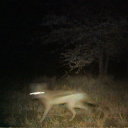
\includegraphics{gfx/diffusion-sampling-loss-guided-vs-correction-guided-qual/diffusion-correction-guided_S2_B06_R1_PICT0128.png} & 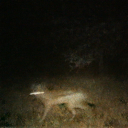
\includegraphics{gfx/diffusion-sampling-loss-guided-vs-correction-guided-qual/diffusion-loss-guided_S2_B06_R1_PICT0128.png} & \includegraphics{gfx/diffusion-sampling-loss-guided-vs-correction-guided-qual/nir_S2_B06_R1_PICT0279.jpg} & 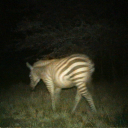
\includegraphics{gfx/diffusion-sampling-loss-guided-vs-correction-guided-qual/diffusion-correction-guided_S2_B06_R1_PICT0279.png} & 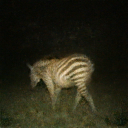
\includegraphics{gfx/diffusion-sampling-loss-guided-vs-correction-guided-qual/diffusion-loss-guided_S2_B06_R1_PICT0279.png} \\
        \includegraphics{gfx/diffusion-sampling-loss-guided-vs-correction-guided-qual/nir_S2_B06_R1_PICT0387.jpg} & 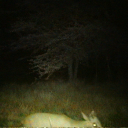
\includegraphics{gfx/diffusion-sampling-loss-guided-vs-correction-guided-qual/diffusion-correction-guided_S2_B06_R1_PICT0387.png} & 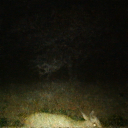
\includegraphics{gfx/diffusion-sampling-loss-guided-vs-correction-guided-qual/diffusion-loss-guided_S2_B06_R1_PICT0387.png} & \includegraphics{gfx/diffusion-sampling-loss-guided-vs-correction-guided-qual/nir_S2_B06_R3_PICT1364.jpg} & 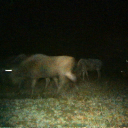
\includegraphics{gfx/diffusion-sampling-loss-guided-vs-correction-guided-qual/diffusion-correction-guided_S2_B06_R3_PICT1364.png} & 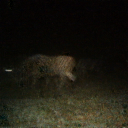
\includegraphics{gfx/diffusion-sampling-loss-guided-vs-correction-guided-qual/diffusion-loss-guided_S2_B06_R3_PICT1364.png} \\
        \includegraphics{gfx/diffusion-sampling-loss-guided-vs-correction-guided-qual/nir_S2_B06_R3_PICT3848.jpg} & 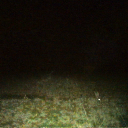
\includegraphics{gfx/diffusion-sampling-loss-guided-vs-correction-guided-qual/diffusion-correction-guided_S2_B06_R3_PICT3848.png} & 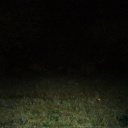
\includegraphics{gfx/diffusion-sampling-loss-guided-vs-correction-guided-qual/diffusion-loss-guided_S2_B06_R3_PICT3848.png} & 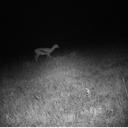
\includegraphics{gfx/diffusion-sampling-loss-guided-vs-correction-guided-qual/nir_S2_B07_R1_PICT3274.jpg} & 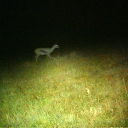
\includegraphics{gfx/diffusion-sampling-loss-guided-vs-correction-guided-qual/diffusion-correction-guided_S2_B07_R1_PICT3274.png} & 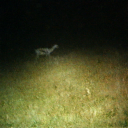
\includegraphics{gfx/diffusion-sampling-loss-guided-vs-correction-guided-qual/diffusion-loss-guided_S2_B07_R1_PICT3274.png}
    \end{tabularx}
    \caption{
        \todo{Add Caption}
    }
    \label{fig:qualitative-evaluation-loss-guided-vs-correction-guided}
\end{figure}

\begin{table}[htp!]
    \centering
    \begin{tabular}{c | c}
        Model             & FID  $\downarrow$ \\
        \hline\hline
        Correction-Guided & 105.00            \\
        Loss-Guided       & 128.64
    \end{tabular}
    \caption{
        \todo{Add Caption}
    }
    \label{fig:quantitative-evaluation-loss-guided-vs-correction-guided}
\end{table}

\todo{Provide intuition for this observation !}

\todo{Unify with observations of \autoref{sec:high-pass-filter-evaluation}}

\section{Conditioning the Near-Infrared}
\subsection{NIR as Intensity Approximation}
\label{sec:nir-as-intensity-approximation-evaluation}
\Textcite{sbgm} already suggested colorization methods using diffusion models.
Although in comparison visible light, near-infrared light has different reflection properties,
we could ignore this property and assume the NIR intensity to be a good approximation of the visual light's intensity.
Therefore, we start by implementing colorization as \autoref{sec:correction-guided-sampling-gray-scale-colorization} and evaluate
this idea empirically.

\begin{figure}[htp!]
    \centering
    \setkeys{Gin}{width=1\linewidth}
    \begin{tabularx}{\textwidth}{Y Y Y !{\space} Y Y Y}
        NIR                                                                                & CycleGAN                                                                                     & Diffusion                                                                                & NIR                                                                                & CycleGAN                                                                                     & Diffusion                                                                                \\
        \includegraphics{gfx/diffusion-sampling-intensity-qual/nir_S2_B06_R1_PICT0128.jpg} & \includegraphics{gfx/diffusion-sampling-intensity-qual/cyclegan_S2_B06_R1_PICT0128_fake.png} & 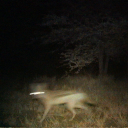
\includegraphics{gfx/diffusion-sampling-intensity-qual/diffusion_S2_B06_R1_PICT0128.png} & \includegraphics{gfx/diffusion-sampling-intensity-qual/nir_S2_B06_R1_PICT0279.jpg} & 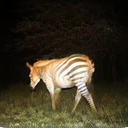
\includegraphics{gfx/diffusion-sampling-intensity-qual/cyclegan_S2_B06_R1_PICT0279_fake.png} & 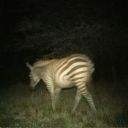
\includegraphics{gfx/diffusion-sampling-intensity-qual/diffusion_S2_B06_R1_PICT0279.png} \\
        \includegraphics{gfx/diffusion-sampling-intensity-qual/nir_S2_B06_R1_PICT0387.jpg} & \includegraphics{gfx/diffusion-sampling-intensity-qual/cyclegan_S2_B06_R1_PICT0387_fake.png} & 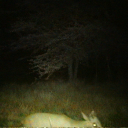
\includegraphics{gfx/diffusion-sampling-intensity-qual/diffusion_S2_B06_R1_PICT0387.png} & \includegraphics{gfx/diffusion-sampling-intensity-qual/nir_S2_B06_R3_PICT1364.jpg} & \includegraphics{gfx/diffusion-sampling-intensity-qual/cyclegan_S2_B06_R3_PICT1364_fake.png} & 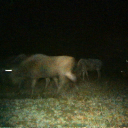
\includegraphics{gfx/diffusion-sampling-intensity-qual/diffusion_S2_B06_R3_PICT1364.png} \\
        \includegraphics{gfx/diffusion-sampling-intensity-qual/nir_S2_B06_R3_PICT3848.jpg} & 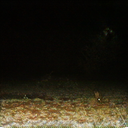
\includegraphics{gfx/diffusion-sampling-intensity-qual/cyclegan_S2_B06_R3_PICT3848_fake.png} & \includegraphics{gfx/diffusion-sampling-intensity-qual/diffusion_S2_B06_R3_PICT3848.png} & \includegraphics{gfx/diffusion-sampling-intensity-qual/nir_S2_B07_R1_PICT3274.jpg} & \includegraphics{gfx/diffusion-sampling-intensity-qual/cyclegan_S2_B07_R1_PICT3274_fake.png} & \includegraphics{gfx/diffusion-sampling-intensity-qual/diffusion_S2_B07_R1_PICT3274.png}
    \end{tabularx}
    \caption{
        \textbf{Qualitative Evaluation.} Left to right: Image from the NIR domain of the Serengeti test dataset \parencite{serengeti},
        corresponding image generated by CycleGAN \parencite{mehri} and corresponding sample generated by our diffusion model approach.
    }
    \label{fig:qualitative-evaluation-intensity}
\end{figure}

In \autoref{fig:qualitative-evaluation-intensity} we show evaluation results of this approach.
Qualitatively we can observe those generated images are faithful to the input image (\autoref{fig:qualitative-evaluation-intensity}).
It is to be mentioned that faithfulness to the input image is not a quality learned by the network, but a design choice of the sampling procedure.
Most noteworthy is that the colors estimated by the diffusion model appear realistic.
Qualitative weaknesses in the colorization can be observed when analyzing the zebra image:
While CycleGAN colorizes the main zebra body as black and white, the diffusion network produces an orange-black zebra.
This can be traced back to a conceptional weakness.
The diffusion network is forced to reuse the intensity of the NIR image.
The zebra in the NIR image is gray-black and therefore the network is not capable in generating high intensity pixels.
CycleGAN on the other-hand is not restricted by design to change the intensity.
It is merely trained to produce invertible images.

\begin{table}[htp!]
    \centering
    \begin{tabular}{c | c}
        Model                                           & FID  $\downarrow$ \\
        \hline\hline
        CycleGAN                                        & 98.10             \\
        Unconditional Diffusion                         & 96.03             \\
        \textbf{Conditional Diffusion} \parencite{sbgm} & \textbf{105.00}
    \end{tabular}
    \caption{
        \textbf{Quantitative Evaluation.} CycleGAN and the diffusion model trained on Snapshot Serengeti \parencite{serengeti} containing only night NIR and RGB images.
        Comparing the FID calculated between the test dataset and the generated images.
    }
    \label{fig:qualitative-evaluation-full-high-pass}
\end{table}


Similar to the minor qualitative weakness, we also observe the FID of this naive approach to be $6.9$ FID points worse than CycleGAN.
Additionally, we see a gap between the sampling the unconditional diffusion model produces our method according to \Citeauthor*{sbgm} of $8.97$ FID points \parencite{sbgm}.
This indicates that this method is too restrictive to allow competitive image generation.


\todo{Explanation why approximation even works, night, few vegetation, ...}

To improve the intuition of the difference between the intensities, we consider CycleGAN's intensities a good approximation of the real visible intensity.
We compare this with the near-infrared intensity in \autoref{fig:heatmap-cycle-gan-intensity}.

\begin{figure}[htp!]
    \centering
    \includegraphics[width=\textwidth]{gfx/heatmap-nir-cycle-gan-intensity-diff.pdf}
    \caption{
        \todo{Better integration (using pdf or so); Best: Direct latex code}
        Absolute difference between CycleGAN's intensity and the NIR image.
        Left to Right: Intensity calculated by images generated by CycleGAN, Near-Infared image \parencite{serengeti} and difference between both.
    }
    \label{fig:heatmap-cycle-gan-intensity}
\end{figure}

We first observe the pattern, that CycleGAN does especially enlighten the foreground and with that the lower regions of the image.
The same holds for animals in the foreground such as the fox or zebra.
Indeed, while comparing the intensity of near-infrared and the incandescent image in the Serengeti dataset \parencite{serengeti}
this pattern is observable again:
Generally the light in incandescent images appears to be stronger and therefore foreground objects are more illuminated.

Naturally when fixing the intensity of the NIR image for the diffusion sampling, such distinct features of the incandescent images is not achievable,
and therefore a higher FID is not unexpected.

As it is now clear that this physical inaccuracy we accepted, might influence the performance of our sampling, it is not yet clear to what extent.
To investigate this, in \autoref{fig:qualitative-evaluation-cyclegan-conditional-sampling} choose to use the same sampling method as before, but instead use the intensities produced by CycleGAN as input to the diffusion sampling.

\begin{figure}[htp!]
    \centering
    \setkeys{Gin}{width=1\linewidth}
    \begin{tabularx}{\textwidth}{Y Y Y !{\space} Y Y Y}
        NIR                                                                              & CycleGAN                                                                                   & Diffusion with CycleGAN Input                                                                    & NIR                                                                              & CycleGAN                                                                                   & Diffusion with CycleGAN Input                                                                    \\
        \includegraphics{gfx/conditional-with-cycle-gan-qual/nir_S2_B06_R1_PICT0128.jpg} & \includegraphics{gfx/conditional-with-cycle-gan-qual/cyclegan_S2_B06_R1_PICT0128_fake.png} & \includegraphics{gfx/conditional-with-cycle-gan-qual/diff_cycle_gan_S2_B06_R1_PICT0128_fake.png} & \includegraphics{gfx/conditional-with-cycle-gan-qual/nir_S2_B06_R1_PICT0279.jpg} & \includegraphics{gfx/conditional-with-cycle-gan-qual/cyclegan_S2_B06_R1_PICT0279_fake.png} & \includegraphics{gfx/conditional-with-cycle-gan-qual/diff_cycle_gan_S2_B06_R1_PICT0279_fake.png} \\
        \includegraphics{gfx/conditional-with-cycle-gan-qual/nir_S2_B06_R1_PICT0387.jpg} & \includegraphics{gfx/conditional-with-cycle-gan-qual/cyclegan_S2_B06_R1_PICT0387_fake.png} & \includegraphics{gfx/conditional-with-cycle-gan-qual/diff_cycle_gan_S2_B06_R1_PICT0387_fake.png} & \includegraphics{gfx/conditional-with-cycle-gan-qual/nir_S2_B06_R3_PICT1364.jpg} & \includegraphics{gfx/conditional-with-cycle-gan-qual/cyclegan_S2_B06_R3_PICT1364_fake.png} & \includegraphics{gfx/conditional-with-cycle-gan-qual/diff_cycle_gan_S2_B06_R3_PICT1364_fake.png} \\
        \includegraphics{gfx/conditional-with-cycle-gan-qual/nir_S2_B06_R3_PICT3848.jpg} & \includegraphics{gfx/conditional-with-cycle-gan-qual/cyclegan_S2_B06_R3_PICT3848_fake.png} & \includegraphics{gfx/conditional-with-cycle-gan-qual/diff_cycle_gan_S2_B06_R3_PICT3848_fake.png} & \includegraphics{gfx/conditional-with-cycle-gan-qual/nir_S2_B07_R1_PICT3274.jpg} & \includegraphics{gfx/conditional-with-cycle-gan-qual/cyclegan_S2_B07_R1_PICT3274_fake.png} & \includegraphics{gfx/conditional-with-cycle-gan-qual/diff_cycle_gan_S2_B07_R1_PICT3274_fake.png}
    \end{tabularx}
    \caption{
        \todo{Add caption}
    }
    \label{fig:qualitative-evaluation-cyclegan-conditional-sampling}
\end{figure}

\begin{table}[htp!]
    \centering
    \begin{tabular}{c | c}
        Model                                    & FID  $\downarrow$ \\
        \hline\hline
        CycleGAN                                 & 98.10             \\
        Diffusion with CycleGAN Intensity Inputs & \textbf{97.21}    \\
        Diffusion with NIR Inputs                & 104.04
    \end{tabular}
    \caption{
        \todo{Add caption}
    }
    \label{fig:quantitative-evaluation-cyclegan-conditional-sampling}
\end{table}


In \autoref{fig:qualitative-evaluation-cyclegan-conditional-sampling} we see that not only is the diffusion model more than capable in colorizing these pictures,
it also exceeds CycleGAN's color choices. While the zebra of CycleGAN has an orange outline at the head where it should not, the diffusion model does not make this mistake
which results in overall more realistic images.

This subtle difference between the CycleGAN and the diffusion model samples with CycleGAN intensity inputs is also visible while comparing the images quantitatively in \autoref{fig:quantitative-evaluation-cyclegan-conditional-sampling}.
The diffusion model performs better than CycleGAN when the intensities are appropriate.
Diffusion models theoretically perform best in the unconditional sampling in comparison when they being guided by unseen data.
In the unconditional setting it only performs $1.2$ FID points better (\autoref{fig:quantitative-evaluation-unconditional-sampling}).
Therefore, we have shown that the assumption that the near-infrared intensities approximate the visual intensities well,
is the main factor explaining the difference between the quantitative results.

\subsection{High-Pass Filtering of NIR}
\label{sec:high-pass-filter-evaluation}

To improve this weakness, we can get inspired by simple NIR-RGB enhancement methods based on filters \parencite{rgb-nir-image-enhancement}.
A better approximation is to use only the high-frequencies of the near-infrared image while the low frequencies can still be sampled by the diffusion model (\autoref{sec:correction-guided-sampling-nir-colorization}).
This intuitively also gives the diffusion model freedom to sample different illumination than given by the near-infrared image.

In \autoref{fig:qualitative-evaluation-full-high-pass} we evaluate the results of this concept.

\begin{figure}[htp!]
    \centering
    \setkeys{Gin}{width=1\linewidth}
    \begin{tabularx}{\textwidth}{Y Y Y !{\space} Y Y Y}
        NIR                                                                                               & Full-Pass                                                                                               & High-Pass                                                                                               & NIR                                                                                               & Full-Pass                                                                                               & High-Pass                                                                                               \\
        \includegraphics{gfx/diffusion-sampling-full-vs-high-pass-filter-qual/nir_S2_B06_R1_PICT0128.jpg} & \includegraphics{gfx/diffusion-sampling-full-vs-high-pass-filter-qual/full-pass_S2_B06_R1_PICT0128.png} & \includegraphics{gfx/diffusion-sampling-full-vs-high-pass-filter-qual/high-pass_S2_B06_R1_PICT0128.png} & \includegraphics{gfx/diffusion-sampling-full-vs-high-pass-filter-qual/nir_S2_B06_R1_PICT0279.jpg} & \includegraphics{gfx/diffusion-sampling-full-vs-high-pass-filter-qual/full-pass_S2_B06_R1_PICT0279.png} & \includegraphics{gfx/diffusion-sampling-full-vs-high-pass-filter-qual/high-pass_S2_B06_R1_PICT0279.png} \\
        \includegraphics{gfx/diffusion-sampling-full-vs-high-pass-filter-qual/nir_S2_B06_R1_PICT0387.jpg} & \includegraphics{gfx/diffusion-sampling-full-vs-high-pass-filter-qual/full-pass_S2_B06_R1_PICT0387.png} & \includegraphics{gfx/diffusion-sampling-full-vs-high-pass-filter-qual/high-pass_S2_B06_R1_PICT0387.png} & \includegraphics{gfx/diffusion-sampling-full-vs-high-pass-filter-qual/nir_S2_B06_R3_PICT1364.jpg} & \includegraphics{gfx/diffusion-sampling-full-vs-high-pass-filter-qual/full-pass_S2_B06_R3_PICT1364.png} & \includegraphics{gfx/diffusion-sampling-full-vs-high-pass-filter-qual/high-pass_S2_B06_R3_PICT1364.png} \\
        \includegraphics{gfx/diffusion-sampling-full-vs-high-pass-filter-qual/nir_S2_B06_R3_PICT3848.jpg} & \includegraphics{gfx/diffusion-sampling-full-vs-high-pass-filter-qual/full-pass_S2_B06_R3_PICT3848.png} & \includegraphics{gfx/diffusion-sampling-full-vs-high-pass-filter-qual/high-pass_S2_B06_R3_PICT3848.png} & \includegraphics{gfx/diffusion-sampling-full-vs-high-pass-filter-qual/nir_S2_B07_R1_PICT3274.jpg} & \includegraphics{gfx/diffusion-sampling-full-vs-high-pass-filter-qual/full-pass_S2_B07_R1_PICT3274.png} & \includegraphics{gfx/diffusion-sampling-full-vs-high-pass-filter-qual/high-pass_S2_B07_R1_PICT3274.png}
    \end{tabularx}
    \caption{
        \todo{Add caption}
    }
    \label{fig:qualitative-evaluation-full-high-pass}
\end{figure}

\begin{table}[htp!]
    \centering
    \begin{tabular}{c | c}
        Strategy      & FID  $\downarrow$ \\
        \hline\hline
        Full-Pass     & 105.00            \\
        High-Pass     & 95.49             \\
        Unconditional & 96.02
    \end{tabular}
    \caption{
        \todo{Add caption}
    }
    \label{fig:quantitative-evaluation-full-high-pass}
\end{table}


As expected the diffusion now using the high-pass filter can manipulate the illumination of the scene.
For example, we observe for left top image now, that not only the fox itself but also the environment has an orange-lighting as typically found in the training dataset.
This reduction in restriction also positively influences the quantitative measurements:
This method achieves a FID of $95.49$ which is even $0.53$ FID points better than the unconditional sampling (\autoref{fig:quantitative-evaluation-full-high-pass}).

\todo{Resolve conflict to statement: "unconditional sampling is always the best" }

\todo{Discuss the qualitative negative points $\rightarrow$ hallucinations}

\subsection{Influence of Hyperparameter Sigma}
\label{sec:influence-of-sigma-evaluation}

While introducing the hyperparameter $\sigma$ in \autoref{sec:correction-guided-sampling-nir-colorization}, we further want to discuss its influence on the samples.
As $\sigma$ controls the strength of the Gaussian-filter for the low-frequency extraction, increasing it, reduces information in the extracted low-frequencies.
Vice versa $\sigma$ raising $\sigma$, leads to more information in the extracted high-frequencies.
We visualize this effect in \autoref{fig:low-and-high-freq-effects-of-sigma}.


\begin{figure}[htp!]
    \centering
    \setkeys{Gin}{width=1\linewidth}
    \begin{tabularx}{.6\textwidth}{>{\centering\arraybackslash}m{.08\linewidth} Y Y Y}
                                                                    & $\sigma=1$                                                           & $\sigma=5$                                                           & $\sigma=10$                                                           \\
        \begin{sideways}\makecell{Low-\\Frequencies}\end{sideways}  & \includegraphics{gfx/low-high-freq-effects-of-sigma/low_freq_1.png}  & \includegraphics{gfx/low-high-freq-effects-of-sigma/low_freq_5.png}  & \includegraphics{gfx/low-high-freq-effects-of-sigma/low_freq_10.png}  \\
        \begin{sideways}\makecell{High-\\Frequencies}\end{sideways} & \includegraphics{gfx/low-high-freq-effects-of-sigma/high_freq_1.png} & \includegraphics{gfx/low-high-freq-effects-of-sigma/high_freq_5.png} & \includegraphics{gfx/low-high-freq-effects-of-sigma/high_freq_10.png} \\
    \end{tabularx}

    \caption{Visualization of different $\sigma$s}
    \label{fig:low-and-high-freq-effects-of-sigma}
\end{figure}

Recall, high-frequency intensities of the near-infrared are combined with the generated low-frequency intensities.
Therefore, a higher $\sigma$ also corresponds to more guidance by the near-infrared image.
On the other hand lower $\sigma$ corresponds to more freedom in generation for the model.
Furthermore one might expect, lower $\sigma$s to correspond to lower and better FIDs, while higher $\sigma$ should
also correspond to higher FIDs and more content preservation.

In \autoref{fig:quantitative-evaluation-influence-of-sigma-to-fid} we visualize the effects of $\sigma$.
All samplings have the same seed, therefore all intermediate samples are the same for all runs.

\begin{figure}[htp!]
    \begin{center}
        %% Creator: Matplotlib, PGF backend
%%
%% To include the figure in your LaTeX document, write
%%   \input{<filename>.pgf}
%%
%% Make sure the required packages are loaded in your preamble
%%   \usepackage{pgf}
%%
%% Also ensure that all the required font packages are loaded; for instance,
%% the lmodern package is sometimes necessary when using math font.
%%   \usepackage{lmodern}
%%
%% Figures using additional raster images can only be included by \input if
%% they are in the same directory as the main LaTeX file. For loading figures
%% from other directories you can use the `import` package
%%   \usepackage{import}
%%
%% and then include the figures with
%%   \import{<path to file>}{<filename>.pgf}
%%
%% Matplotlib used the following preamble
%%   \usepackage{fontspec}
%%
\begingroup%
\makeatletter%
\begin{pgfpicture}%
\pgfpathrectangle{\pgfpointorigin}{\pgfqpoint{6.400000in}{4.800000in}}%
\pgfusepath{use as bounding box, clip}%
\begin{pgfscope}%
\pgfsetbuttcap%
\pgfsetmiterjoin%
\definecolor{currentfill}{rgb}{1.000000,1.000000,1.000000}%
\pgfsetfillcolor{currentfill}%
\pgfsetlinewidth{0.000000pt}%
\definecolor{currentstroke}{rgb}{1.000000,1.000000,1.000000}%
\pgfsetstrokecolor{currentstroke}%
\pgfsetdash{}{0pt}%
\pgfpathmoveto{\pgfqpoint{0.000000in}{0.000000in}}%
\pgfpathlineto{\pgfqpoint{6.400000in}{0.000000in}}%
\pgfpathlineto{\pgfqpoint{6.400000in}{4.800000in}}%
\pgfpathlineto{\pgfqpoint{0.000000in}{4.800000in}}%
\pgfpathlineto{\pgfqpoint{0.000000in}{0.000000in}}%
\pgfpathclose%
\pgfusepath{fill}%
\end{pgfscope}%
\begin{pgfscope}%
\pgfsetbuttcap%
\pgfsetmiterjoin%
\definecolor{currentfill}{rgb}{1.000000,1.000000,1.000000}%
\pgfsetfillcolor{currentfill}%
\pgfsetlinewidth{0.000000pt}%
\definecolor{currentstroke}{rgb}{0.000000,0.000000,0.000000}%
\pgfsetstrokecolor{currentstroke}%
\pgfsetstrokeopacity{0.000000}%
\pgfsetdash{}{0pt}%
\pgfpathmoveto{\pgfqpoint{0.800000in}{0.528000in}}%
\pgfpathlineto{\pgfqpoint{5.760000in}{0.528000in}}%
\pgfpathlineto{\pgfqpoint{5.760000in}{4.224000in}}%
\pgfpathlineto{\pgfqpoint{0.800000in}{4.224000in}}%
\pgfpathlineto{\pgfqpoint{0.800000in}{0.528000in}}%
\pgfpathclose%
\pgfusepath{fill}%
\end{pgfscope}%
\begin{pgfscope}%
\pgfpathrectangle{\pgfqpoint{0.800000in}{0.528000in}}{\pgfqpoint{4.960000in}{3.696000in}}%
\pgfusepath{clip}%
\pgfsetroundcap%
\pgfsetroundjoin%
\pgfsetlinewidth{0.803000pt}%
\definecolor{currentstroke}{rgb}{0.800000,0.800000,0.800000}%
\pgfsetstrokecolor{currentstroke}%
\pgfsetdash{}{0pt}%
\pgfpathmoveto{\pgfqpoint{1.556610in}{0.528000in}}%
\pgfpathlineto{\pgfqpoint{1.556610in}{4.224000in}}%
\pgfusepath{stroke}%
\end{pgfscope}%
\begin{pgfscope}%
\definecolor{textcolor}{rgb}{0.150000,0.150000,0.150000}%
\pgfsetstrokecolor{textcolor}%
\pgfsetfillcolor{textcolor}%
\pgftext[x=1.556610in,y=0.412722in,,top]{\color{textcolor}\rmfamily\fontsize{8.800000}{10.560000}\selectfont \(\displaystyle {5}\)}%
\end{pgfscope}%
\begin{pgfscope}%
\pgfpathrectangle{\pgfqpoint{0.800000in}{0.528000in}}{\pgfqpoint{4.960000in}{3.696000in}}%
\pgfusepath{clip}%
\pgfsetroundcap%
\pgfsetroundjoin%
\pgfsetlinewidth{0.803000pt}%
\definecolor{currentstroke}{rgb}{0.800000,0.800000,0.800000}%
\pgfsetstrokecolor{currentstroke}%
\pgfsetdash{}{0pt}%
\pgfpathmoveto{\pgfqpoint{2.397288in}{0.528000in}}%
\pgfpathlineto{\pgfqpoint{2.397288in}{4.224000in}}%
\pgfusepath{stroke}%
\end{pgfscope}%
\begin{pgfscope}%
\definecolor{textcolor}{rgb}{0.150000,0.150000,0.150000}%
\pgfsetstrokecolor{textcolor}%
\pgfsetfillcolor{textcolor}%
\pgftext[x=2.397288in,y=0.412722in,,top]{\color{textcolor}\rmfamily\fontsize{8.800000}{10.560000}\selectfont \(\displaystyle {10}\)}%
\end{pgfscope}%
\begin{pgfscope}%
\pgfpathrectangle{\pgfqpoint{0.800000in}{0.528000in}}{\pgfqpoint{4.960000in}{3.696000in}}%
\pgfusepath{clip}%
\pgfsetroundcap%
\pgfsetroundjoin%
\pgfsetlinewidth{0.803000pt}%
\definecolor{currentstroke}{rgb}{0.800000,0.800000,0.800000}%
\pgfsetstrokecolor{currentstroke}%
\pgfsetdash{}{0pt}%
\pgfpathmoveto{\pgfqpoint{3.237966in}{0.528000in}}%
\pgfpathlineto{\pgfqpoint{3.237966in}{4.224000in}}%
\pgfusepath{stroke}%
\end{pgfscope}%
\begin{pgfscope}%
\definecolor{textcolor}{rgb}{0.150000,0.150000,0.150000}%
\pgfsetstrokecolor{textcolor}%
\pgfsetfillcolor{textcolor}%
\pgftext[x=3.237966in,y=0.412722in,,top]{\color{textcolor}\rmfamily\fontsize{8.800000}{10.560000}\selectfont \(\displaystyle {15}\)}%
\end{pgfscope}%
\begin{pgfscope}%
\pgfpathrectangle{\pgfqpoint{0.800000in}{0.528000in}}{\pgfqpoint{4.960000in}{3.696000in}}%
\pgfusepath{clip}%
\pgfsetroundcap%
\pgfsetroundjoin%
\pgfsetlinewidth{0.803000pt}%
\definecolor{currentstroke}{rgb}{0.800000,0.800000,0.800000}%
\pgfsetstrokecolor{currentstroke}%
\pgfsetdash{}{0pt}%
\pgfpathmoveto{\pgfqpoint{4.078644in}{0.528000in}}%
\pgfpathlineto{\pgfqpoint{4.078644in}{4.224000in}}%
\pgfusepath{stroke}%
\end{pgfscope}%
\begin{pgfscope}%
\definecolor{textcolor}{rgb}{0.150000,0.150000,0.150000}%
\pgfsetstrokecolor{textcolor}%
\pgfsetfillcolor{textcolor}%
\pgftext[x=4.078644in,y=0.412722in,,top]{\color{textcolor}\rmfamily\fontsize{8.800000}{10.560000}\selectfont \(\displaystyle {20}\)}%
\end{pgfscope}%
\begin{pgfscope}%
\pgfpathrectangle{\pgfqpoint{0.800000in}{0.528000in}}{\pgfqpoint{4.960000in}{3.696000in}}%
\pgfusepath{clip}%
\pgfsetroundcap%
\pgfsetroundjoin%
\pgfsetlinewidth{0.803000pt}%
\definecolor{currentstroke}{rgb}{0.800000,0.800000,0.800000}%
\pgfsetstrokecolor{currentstroke}%
\pgfsetdash{}{0pt}%
\pgfpathmoveto{\pgfqpoint{4.919322in}{0.528000in}}%
\pgfpathlineto{\pgfqpoint{4.919322in}{4.224000in}}%
\pgfusepath{stroke}%
\end{pgfscope}%
\begin{pgfscope}%
\definecolor{textcolor}{rgb}{0.150000,0.150000,0.150000}%
\pgfsetstrokecolor{textcolor}%
\pgfsetfillcolor{textcolor}%
\pgftext[x=4.919322in,y=0.412722in,,top]{\color{textcolor}\rmfamily\fontsize{8.800000}{10.560000}\selectfont \(\displaystyle {25}\)}%
\end{pgfscope}%
\begin{pgfscope}%
\pgfpathrectangle{\pgfqpoint{0.800000in}{0.528000in}}{\pgfqpoint{4.960000in}{3.696000in}}%
\pgfusepath{clip}%
\pgfsetroundcap%
\pgfsetroundjoin%
\pgfsetlinewidth{0.803000pt}%
\definecolor{currentstroke}{rgb}{0.800000,0.800000,0.800000}%
\pgfsetstrokecolor{currentstroke}%
\pgfsetdash{}{0pt}%
\pgfpathmoveto{\pgfqpoint{5.760000in}{0.528000in}}%
\pgfpathlineto{\pgfqpoint{5.760000in}{4.224000in}}%
\pgfusepath{stroke}%
\end{pgfscope}%
\begin{pgfscope}%
\definecolor{textcolor}{rgb}{0.150000,0.150000,0.150000}%
\pgfsetstrokecolor{textcolor}%
\pgfsetfillcolor{textcolor}%
\pgftext[x=5.760000in,y=0.412722in,,top]{\color{textcolor}\rmfamily\fontsize{8.800000}{10.560000}\selectfont \(\displaystyle {30}\)}%
\end{pgfscope}%
\begin{pgfscope}%
\definecolor{textcolor}{rgb}{0.150000,0.150000,0.150000}%
\pgfsetstrokecolor{textcolor}%
\pgfsetfillcolor{textcolor}%
\pgftext[x=3.280000in,y=0.248633in,,top]{\color{textcolor}\rmfamily\fontsize{9.600000}{11.520000}\selectfont \(\displaystyle \sigma\)}%
\end{pgfscope}%
\begin{pgfscope}%
\pgfpathrectangle{\pgfqpoint{0.800000in}{0.528000in}}{\pgfqpoint{4.960000in}{3.696000in}}%
\pgfusepath{clip}%
\pgfsetroundcap%
\pgfsetroundjoin%
\pgfsetlinewidth{0.803000pt}%
\definecolor{currentstroke}{rgb}{0.800000,0.800000,0.800000}%
\pgfsetstrokecolor{currentstroke}%
\pgfsetdash{}{0pt}%
\pgfpathmoveto{\pgfqpoint{0.800000in}{0.528000in}}%
\pgfpathlineto{\pgfqpoint{5.760000in}{0.528000in}}%
\pgfusepath{stroke}%
\end{pgfscope}%
\begin{pgfscope}%
\definecolor{textcolor}{rgb}{0.150000,0.150000,0.150000}%
\pgfsetstrokecolor{textcolor}%
\pgfsetfillcolor{textcolor}%
\pgftext[x=0.556251in, y=0.485589in, left, base]{\color{textcolor}\rmfamily\fontsize{8.800000}{10.560000}\selectfont \(\displaystyle {94}\)}%
\end{pgfscope}%
\begin{pgfscope}%
\pgfpathrectangle{\pgfqpoint{0.800000in}{0.528000in}}{\pgfqpoint{4.960000in}{3.696000in}}%
\pgfusepath{clip}%
\pgfsetroundcap%
\pgfsetroundjoin%
\pgfsetlinewidth{0.803000pt}%
\definecolor{currentstroke}{rgb}{0.800000,0.800000,0.800000}%
\pgfsetstrokecolor{currentstroke}%
\pgfsetdash{}{0pt}%
\pgfpathmoveto{\pgfqpoint{0.800000in}{1.144000in}}%
\pgfpathlineto{\pgfqpoint{5.760000in}{1.144000in}}%
\pgfusepath{stroke}%
\end{pgfscope}%
\begin{pgfscope}%
\definecolor{textcolor}{rgb}{0.150000,0.150000,0.150000}%
\pgfsetstrokecolor{textcolor}%
\pgfsetfillcolor{textcolor}%
\pgftext[x=0.556251in, y=1.101589in, left, base]{\color{textcolor}\rmfamily\fontsize{8.800000}{10.560000}\selectfont \(\displaystyle {96}\)}%
\end{pgfscope}%
\begin{pgfscope}%
\pgfpathrectangle{\pgfqpoint{0.800000in}{0.528000in}}{\pgfqpoint{4.960000in}{3.696000in}}%
\pgfusepath{clip}%
\pgfsetroundcap%
\pgfsetroundjoin%
\pgfsetlinewidth{0.803000pt}%
\definecolor{currentstroke}{rgb}{0.800000,0.800000,0.800000}%
\pgfsetstrokecolor{currentstroke}%
\pgfsetdash{}{0pt}%
\pgfpathmoveto{\pgfqpoint{0.800000in}{1.760000in}}%
\pgfpathlineto{\pgfqpoint{5.760000in}{1.760000in}}%
\pgfusepath{stroke}%
\end{pgfscope}%
\begin{pgfscope}%
\definecolor{textcolor}{rgb}{0.150000,0.150000,0.150000}%
\pgfsetstrokecolor{textcolor}%
\pgfsetfillcolor{textcolor}%
\pgftext[x=0.556251in, y=1.717589in, left, base]{\color{textcolor}\rmfamily\fontsize{8.800000}{10.560000}\selectfont \(\displaystyle {98}\)}%
\end{pgfscope}%
\begin{pgfscope}%
\pgfpathrectangle{\pgfqpoint{0.800000in}{0.528000in}}{\pgfqpoint{4.960000in}{3.696000in}}%
\pgfusepath{clip}%
\pgfsetroundcap%
\pgfsetroundjoin%
\pgfsetlinewidth{0.803000pt}%
\definecolor{currentstroke}{rgb}{0.800000,0.800000,0.800000}%
\pgfsetstrokecolor{currentstroke}%
\pgfsetdash{}{0pt}%
\pgfpathmoveto{\pgfqpoint{0.800000in}{2.376000in}}%
\pgfpathlineto{\pgfqpoint{5.760000in}{2.376000in}}%
\pgfusepath{stroke}%
\end{pgfscope}%
\begin{pgfscope}%
\definecolor{textcolor}{rgb}{0.150000,0.150000,0.150000}%
\pgfsetstrokecolor{textcolor}%
\pgfsetfillcolor{textcolor}%
\pgftext[x=0.492015in, y=2.333589in, left, base]{\color{textcolor}\rmfamily\fontsize{8.800000}{10.560000}\selectfont \(\displaystyle {100}\)}%
\end{pgfscope}%
\begin{pgfscope}%
\pgfpathrectangle{\pgfqpoint{0.800000in}{0.528000in}}{\pgfqpoint{4.960000in}{3.696000in}}%
\pgfusepath{clip}%
\pgfsetroundcap%
\pgfsetroundjoin%
\pgfsetlinewidth{0.803000pt}%
\definecolor{currentstroke}{rgb}{0.800000,0.800000,0.800000}%
\pgfsetstrokecolor{currentstroke}%
\pgfsetdash{}{0pt}%
\pgfpathmoveto{\pgfqpoint{0.800000in}{2.992000in}}%
\pgfpathlineto{\pgfqpoint{5.760000in}{2.992000in}}%
\pgfusepath{stroke}%
\end{pgfscope}%
\begin{pgfscope}%
\definecolor{textcolor}{rgb}{0.150000,0.150000,0.150000}%
\pgfsetstrokecolor{textcolor}%
\pgfsetfillcolor{textcolor}%
\pgftext[x=0.492015in, y=2.949589in, left, base]{\color{textcolor}\rmfamily\fontsize{8.800000}{10.560000}\selectfont \(\displaystyle {102}\)}%
\end{pgfscope}%
\begin{pgfscope}%
\pgfpathrectangle{\pgfqpoint{0.800000in}{0.528000in}}{\pgfqpoint{4.960000in}{3.696000in}}%
\pgfusepath{clip}%
\pgfsetroundcap%
\pgfsetroundjoin%
\pgfsetlinewidth{0.803000pt}%
\definecolor{currentstroke}{rgb}{0.800000,0.800000,0.800000}%
\pgfsetstrokecolor{currentstroke}%
\pgfsetdash{}{0pt}%
\pgfpathmoveto{\pgfqpoint{0.800000in}{3.608000in}}%
\pgfpathlineto{\pgfqpoint{5.760000in}{3.608000in}}%
\pgfusepath{stroke}%
\end{pgfscope}%
\begin{pgfscope}%
\definecolor{textcolor}{rgb}{0.150000,0.150000,0.150000}%
\pgfsetstrokecolor{textcolor}%
\pgfsetfillcolor{textcolor}%
\pgftext[x=0.492015in, y=3.565589in, left, base]{\color{textcolor}\rmfamily\fontsize{8.800000}{10.560000}\selectfont \(\displaystyle {104}\)}%
\end{pgfscope}%
\begin{pgfscope}%
\pgfpathrectangle{\pgfqpoint{0.800000in}{0.528000in}}{\pgfqpoint{4.960000in}{3.696000in}}%
\pgfusepath{clip}%
\pgfsetroundcap%
\pgfsetroundjoin%
\pgfsetlinewidth{0.803000pt}%
\definecolor{currentstroke}{rgb}{0.800000,0.800000,0.800000}%
\pgfsetstrokecolor{currentstroke}%
\pgfsetdash{}{0pt}%
\pgfpathmoveto{\pgfqpoint{0.800000in}{4.224000in}}%
\pgfpathlineto{\pgfqpoint{5.760000in}{4.224000in}}%
\pgfusepath{stroke}%
\end{pgfscope}%
\begin{pgfscope}%
\definecolor{textcolor}{rgb}{0.150000,0.150000,0.150000}%
\pgfsetstrokecolor{textcolor}%
\pgfsetfillcolor{textcolor}%
\pgftext[x=0.492015in, y=4.181589in, left, base]{\color{textcolor}\rmfamily\fontsize{8.800000}{10.560000}\selectfont \(\displaystyle {106}\)}%
\end{pgfscope}%
\begin{pgfscope}%
\definecolor{textcolor}{rgb}{0.150000,0.150000,0.150000}%
\pgfsetstrokecolor{textcolor}%
\pgfsetfillcolor{textcolor}%
\pgftext[x=0.436460in,y=2.376000in,,bottom,rotate=90.000000]{\color{textcolor}\rmfamily\fontsize{9.600000}{11.520000}\selectfont FID \(\displaystyle \downarrow\)}%
\end{pgfscope}%
\begin{pgfscope}%
\pgfpathrectangle{\pgfqpoint{0.800000in}{0.528000in}}{\pgfqpoint{4.960000in}{3.696000in}}%
\pgfusepath{clip}%
\pgfsetroundcap%
\pgfsetroundjoin%
\pgfsetlinewidth{1.204500pt}%
\definecolor{currentstroke}{rgb}{0.988235,0.729412,0.000000}%
\pgfsetstrokecolor{currentstroke}%
\pgfsetdash{}{0pt}%
\pgfpathmoveto{\pgfqpoint{0.800000in}{1.790920in}}%
\pgfpathlineto{\pgfqpoint{5.760000in}{1.790920in}}%
\pgfusepath{stroke}%
\end{pgfscope}%
\begin{pgfscope}%
\pgfpathrectangle{\pgfqpoint{0.800000in}{0.528000in}}{\pgfqpoint{4.960000in}{3.696000in}}%
\pgfusepath{clip}%
\pgfsetroundcap%
\pgfsetroundjoin%
\pgfsetlinewidth{1.204500pt}%
\definecolor{currentstroke}{rgb}{0.564706,0.564706,0.521569}%
\pgfsetstrokecolor{currentstroke}%
\pgfsetdash{}{0pt}%
\pgfpathmoveto{\pgfqpoint{0.800000in}{1.153235in}}%
\pgfpathlineto{\pgfqpoint{5.760000in}{1.153235in}}%
\pgfusepath{stroke}%
\end{pgfscope}%
\begin{pgfscope}%
\pgfpathrectangle{\pgfqpoint{0.800000in}{0.528000in}}{\pgfqpoint{4.960000in}{3.696000in}}%
\pgfusepath{clip}%
\pgfsetroundcap%
\pgfsetroundjoin%
\pgfsetlinewidth{1.204500pt}%
\definecolor{currentstroke}{rgb}{0.000000,0.305882,0.623529}%
\pgfsetstrokecolor{currentstroke}%
\pgfsetdash{}{0pt}%
\pgfpathmoveto{\pgfqpoint{0.882015in}{4.234000in}}%
\pgfpathlineto{\pgfqpoint{0.884068in}{4.049215in}}%
\pgfpathlineto{\pgfqpoint{0.926102in}{2.557995in}}%
\pgfpathlineto{\pgfqpoint{0.968136in}{1.764717in}}%
\pgfpathlineto{\pgfqpoint{1.010169in}{1.438257in}}%
\pgfpathlineto{\pgfqpoint{1.052203in}{1.335676in}}%
\pgfpathlineto{\pgfqpoint{1.069017in}{1.332455in}}%
\pgfpathlineto{\pgfqpoint{1.085831in}{1.349404in}}%
\pgfpathlineto{\pgfqpoint{1.102644in}{1.323530in}}%
\pgfpathlineto{\pgfqpoint{1.119458in}{1.458855in}}%
\pgfpathlineto{\pgfqpoint{1.136271in}{1.484833in}}%
\pgfpathlineto{\pgfqpoint{1.153085in}{1.486294in}}%
\pgfpathlineto{\pgfqpoint{1.169898in}{1.557503in}}%
\pgfpathlineto{\pgfqpoint{1.186712in}{1.726601in}}%
\pgfpathlineto{\pgfqpoint{1.203525in}{1.759992in}}%
\pgfpathlineto{\pgfqpoint{1.220339in}{1.783199in}}%
\pgfpathlineto{\pgfqpoint{1.262373in}{2.232745in}}%
\pgfpathlineto{\pgfqpoint{1.304407in}{2.319760in}}%
\pgfpathlineto{\pgfqpoint{1.346441in}{2.451358in}}%
\pgfpathlineto{\pgfqpoint{1.388475in}{2.560051in}}%
\pgfpathlineto{\pgfqpoint{1.472542in}{2.628868in}}%
\pgfpathlineto{\pgfqpoint{1.556610in}{2.838007in}}%
\pgfpathlineto{\pgfqpoint{1.724746in}{2.835128in}}%
\pgfpathlineto{\pgfqpoint{1.892881in}{3.030512in}}%
\pgfpathlineto{\pgfqpoint{2.061017in}{3.108897in}}%
\pgfpathlineto{\pgfqpoint{2.229153in}{3.192095in}}%
\pgfpathlineto{\pgfqpoint{2.397288in}{3.284290in}}%
\pgfpathlineto{\pgfqpoint{3.237966in}{3.404216in}}%
\pgfpathlineto{\pgfqpoint{4.078644in}{3.248514in}}%
\pgfpathlineto{\pgfqpoint{4.919322in}{3.244564in}}%
\pgfpathlineto{\pgfqpoint{5.760000in}{3.174719in}}%
\pgfusepath{stroke}%
\end{pgfscope}%
\begin{pgfscope}%
\pgfpathrectangle{\pgfqpoint{0.800000in}{0.528000in}}{\pgfqpoint{4.960000in}{3.696000in}}%
\pgfusepath{clip}%
\pgfsetbuttcap%
\pgfsetroundjoin%
\pgfsetlinewidth{1.204500pt}%
\definecolor{currentstroke}{rgb}{0.000000,0.305882,0.623529}%
\pgfsetstrokecolor{currentstroke}%
\pgfsetdash{{4.440000pt}{1.920000pt}}{0.000000pt}%
\pgfpathmoveto{\pgfqpoint{0.800000in}{3.914587in}}%
\pgfpathlineto{\pgfqpoint{5.760000in}{3.914587in}}%
\pgfusepath{stroke}%
\end{pgfscope}%
\begin{pgfscope}%
\pgfsetrectcap%
\pgfsetmiterjoin%
\pgfsetlinewidth{1.003750pt}%
\definecolor{currentstroke}{rgb}{0.800000,0.800000,0.800000}%
\pgfsetstrokecolor{currentstroke}%
\pgfsetdash{}{0pt}%
\pgfpathmoveto{\pgfqpoint{0.800000in}{0.528000in}}%
\pgfpathlineto{\pgfqpoint{0.800000in}{4.224000in}}%
\pgfusepath{stroke}%
\end{pgfscope}%
\begin{pgfscope}%
\pgfsetrectcap%
\pgfsetmiterjoin%
\pgfsetlinewidth{1.003750pt}%
\definecolor{currentstroke}{rgb}{0.800000,0.800000,0.800000}%
\pgfsetstrokecolor{currentstroke}%
\pgfsetdash{}{0pt}%
\pgfpathmoveto{\pgfqpoint{5.760000in}{0.528000in}}%
\pgfpathlineto{\pgfqpoint{5.760000in}{4.224000in}}%
\pgfusepath{stroke}%
\end{pgfscope}%
\begin{pgfscope}%
\pgfsetrectcap%
\pgfsetmiterjoin%
\pgfsetlinewidth{1.003750pt}%
\definecolor{currentstroke}{rgb}{0.800000,0.800000,0.800000}%
\pgfsetstrokecolor{currentstroke}%
\pgfsetdash{}{0pt}%
\pgfpathmoveto{\pgfqpoint{0.800000in}{0.528000in}}%
\pgfpathlineto{\pgfqpoint{5.760000in}{0.528000in}}%
\pgfusepath{stroke}%
\end{pgfscope}%
\begin{pgfscope}%
\pgfsetrectcap%
\pgfsetmiterjoin%
\pgfsetlinewidth{1.003750pt}%
\definecolor{currentstroke}{rgb}{0.800000,0.800000,0.800000}%
\pgfsetstrokecolor{currentstroke}%
\pgfsetdash{}{0pt}%
\pgfpathmoveto{\pgfqpoint{0.800000in}{4.224000in}}%
\pgfpathlineto{\pgfqpoint{5.760000in}{4.224000in}}%
\pgfusepath{stroke}%
\end{pgfscope}%
\begin{pgfscope}%
\pgfsetbuttcap%
\pgfsetmiterjoin%
\definecolor{currentfill}{rgb}{1.000000,1.000000,1.000000}%
\pgfsetfillcolor{currentfill}%
\pgfsetfillopacity{0.800000}%
\pgfsetlinewidth{0.803000pt}%
\definecolor{currentstroke}{rgb}{0.800000,0.800000,0.800000}%
\pgfsetstrokecolor{currentstroke}%
\pgfsetstrokeopacity{0.800000}%
\pgfsetdash{}{0pt}%
\pgfpathmoveto{\pgfqpoint{3.585698in}{2.013856in}}%
\pgfpathlineto{\pgfqpoint{5.674444in}{2.013856in}}%
\pgfpathquadraticcurveto{\pgfqpoint{5.698889in}{2.013856in}}{\pgfqpoint{5.698889in}{2.038300in}}%
\pgfpathlineto{\pgfqpoint{5.698889in}{2.713700in}}%
\pgfpathquadraticcurveto{\pgfqpoint{5.698889in}{2.738144in}}{\pgfqpoint{5.674444in}{2.738144in}}%
\pgfpathlineto{\pgfqpoint{3.585698in}{2.738144in}}%
\pgfpathquadraticcurveto{\pgfqpoint{3.561254in}{2.738144in}}{\pgfqpoint{3.561254in}{2.713700in}}%
\pgfpathlineto{\pgfqpoint{3.561254in}{2.038300in}}%
\pgfpathquadraticcurveto{\pgfqpoint{3.561254in}{2.013856in}}{\pgfqpoint{3.585698in}{2.013856in}}%
\pgfpathlineto{\pgfqpoint{3.585698in}{2.013856in}}%
\pgfpathclose%
\pgfusepath{stroke,fill}%
\end{pgfscope}%
\begin{pgfscope}%
\pgfsetroundcap%
\pgfsetroundjoin%
\pgfsetlinewidth{1.204500pt}%
\definecolor{currentstroke}{rgb}{0.988235,0.729412,0.000000}%
\pgfsetstrokecolor{currentstroke}%
\pgfsetdash{}{0pt}%
\pgfpathmoveto{\pgfqpoint{3.610143in}{2.644522in}}%
\pgfpathlineto{\pgfqpoint{3.732365in}{2.644522in}}%
\pgfpathlineto{\pgfqpoint{3.854587in}{2.644522in}}%
\pgfusepath{stroke}%
\end{pgfscope}%
\begin{pgfscope}%
\definecolor{textcolor}{rgb}{0.150000,0.150000,0.150000}%
\pgfsetstrokecolor{textcolor}%
\pgfsetfillcolor{textcolor}%
\pgftext[x=3.952365in,y=2.601744in,left,base]{\color{textcolor}\rmfamily\fontsize{8.800000}{10.560000}\selectfont CycleGAN}%
\end{pgfscope}%
\begin{pgfscope}%
\pgfsetroundcap%
\pgfsetroundjoin%
\pgfsetlinewidth{1.204500pt}%
\definecolor{currentstroke}{rgb}{0.564706,0.564706,0.521569}%
\pgfsetstrokecolor{currentstroke}%
\pgfsetdash{}{0pt}%
\pgfpathmoveto{\pgfqpoint{3.610143in}{2.472800in}}%
\pgfpathlineto{\pgfqpoint{3.732365in}{2.472800in}}%
\pgfpathlineto{\pgfqpoint{3.854587in}{2.472800in}}%
\pgfusepath{stroke}%
\end{pgfscope}%
\begin{pgfscope}%
\definecolor{textcolor}{rgb}{0.150000,0.150000,0.150000}%
\pgfsetstrokecolor{textcolor}%
\pgfsetfillcolor{textcolor}%
\pgftext[x=3.952365in,y=2.430022in,left,base]{\color{textcolor}\rmfamily\fontsize{8.800000}{10.560000}\selectfont Unconditional Diffusion}%
\end{pgfscope}%
\begin{pgfscope}%
\pgfsetroundcap%
\pgfsetroundjoin%
\pgfsetlinewidth{1.204500pt}%
\definecolor{currentstroke}{rgb}{0.000000,0.305882,0.623529}%
\pgfsetstrokecolor{currentstroke}%
\pgfsetdash{}{0pt}%
\pgfpathmoveto{\pgfqpoint{3.610143in}{2.302422in}}%
\pgfpathlineto{\pgfqpoint{3.732365in}{2.302422in}}%
\pgfpathlineto{\pgfqpoint{3.854587in}{2.302422in}}%
\pgfusepath{stroke}%
\end{pgfscope}%
\begin{pgfscope}%
\definecolor{textcolor}{rgb}{0.150000,0.150000,0.150000}%
\pgfsetstrokecolor{textcolor}%
\pgfsetfillcolor{textcolor}%
\pgftext[x=3.952365in,y=2.259645in,left,base]{\color{textcolor}\rmfamily\fontsize{8.800000}{10.560000}\selectfont High-Freq Replacement with \(\displaystyle \sigma\)}%
\end{pgfscope}%
\begin{pgfscope}%
\pgfsetbuttcap%
\pgfsetroundjoin%
\pgfsetlinewidth{1.204500pt}%
\definecolor{currentstroke}{rgb}{0.000000,0.305882,0.623529}%
\pgfsetstrokecolor{currentstroke}%
\pgfsetdash{{4.440000pt}{1.920000pt}}{0.000000pt}%
\pgfpathmoveto{\pgfqpoint{3.610143in}{2.130578in}}%
\pgfpathlineto{\pgfqpoint{3.732365in}{2.130578in}}%
\pgfpathlineto{\pgfqpoint{3.854587in}{2.130578in}}%
\pgfusepath{stroke}%
\end{pgfscope}%
\begin{pgfscope}%
\definecolor{textcolor}{rgb}{0.150000,0.150000,0.150000}%
\pgfsetstrokecolor{textcolor}%
\pgfsetfillcolor{textcolor}%
\pgftext[x=3.952365in,y=2.087800in,left,base]{\color{textcolor}\rmfamily\fontsize{8.800000}{10.560000}\selectfont Intensity Replacement}%
\end{pgfscope}%
\end{pgfpicture}%
\makeatother%
\endgroup%

    \end{center}
    \caption{Influence of $\sigma$ to the FID. On the x-axis the FID (lower is better) and on the y-axis the $\sigma$ for the model}
    \label{fig:quantitative-evaluation-influence-of-sigma-to-fid}
\end{figure}



\section{Diffusion and GAN}
\label{sec:diffusion-vs-cyclegan}
To study the difference between diffusion models and generative adversarial networks for near-infrared image colorization, we compare them for two specialized problems.

First we evaluate the performances on the Caltech Camera Traps dataset (\autoref{sec:cct}) by \Citeauthor*{caltech}.
The near-infrared images in the dataset are mostly taken during the night, while the color images are from the daytime \parencite{caltech}.
Both networks are required to translate mostly night near-infrared images to colored images while having mostly seen day images.
This results in artificial difficulty for the networks (\autoref{sec:diffusion-vs-cyclegan-day}).

Secondly we evaluate both networks on a more application-oriented dataset.
The subset of the Serengeti dataset we use consists mostly of night images for the near infrared domain as for the colored domain.
As near-infared applications lie for the most part in generating high-quality night images this is closer to an application context.
Because the networks are not required to perform a translation to colored night images, without having seen many of those, we consider
this specialized problem as easier, which is also visible in the quality of the results (\autoref{sec:diffusion-vs-cyclegan-night})

\subsection{Extended Dataset --- Robustness}
\label{sec:diffusion-vs-cyclegan-day}
Using the Caltech Camera Traps data split we introduced in \autoref{sec:cct},
we train an unconditional diffusion model on the mostly colored daytime images from the training dataset.

Our unconditional model is evaluated first, to validate the model did learn to approximate the target distribution well.
As visible in \autoref{fig:qualitative-evaluation-unconditional-sampling-caltech} qualitatively the diffusion network
produces highly realistic images matching the style and diversity of the test dataset well.
Quantitatively the samples achieve a fréchet inception distance of $100.22$ to the test data set.
Compared with other FIDs in this work we consider it a good value.

\begin{figure}[htp!]
    \centering
    \setkeys{Gin}{width=1\linewidth}
    \begin{tabularx}{\textwidth}{Y Y Y !{\space} Y Y Y !{\space}}
        RGB                                                                                                              & Diffusion                                                                               & RGB                                                                                                              & Diffusion                                                                               & RGB                                                                                                              & Diffusion                                                                               \\
        \includegraphics{gfx/unconditional-diffusion-sampling-caltech-qual/rgb_5858c0dc-23d2-11e8-a6a3-ec086b02610b.jpg} & \includegraphics{gfx/unconditional-diffusion-sampling-caltech-qual/diffusion_00000.png} & \includegraphics{gfx/unconditional-diffusion-sampling-caltech-qual/rgb_585a640e-23d2-11e8-a6a3-ec086b02610b.jpg} & \includegraphics{gfx/unconditional-diffusion-sampling-caltech-qual/diffusion_00001.png} & \includegraphics{gfx/unconditional-diffusion-sampling-caltech-qual/rgb_585a6486-23d2-11e8-a6a3-ec086b02610b.jpg} & \includegraphics{gfx/unconditional-diffusion-sampling-caltech-qual/diffusion_00002.png} \\
        \includegraphics{gfx/unconditional-diffusion-sampling-caltech-qual/rgb_585dab96-23d2-11e8-a6a3-ec086b02610b.jpg} & \includegraphics{gfx/unconditional-diffusion-sampling-caltech-qual/diffusion_00003.png} & \includegraphics{gfx/unconditional-diffusion-sampling-caltech-qual/rgb_585f4d99-23d2-11e8-a6a3-ec086b02610b.jpg} & \includegraphics{gfx/unconditional-diffusion-sampling-caltech-qual/diffusion_00004.png} & \includegraphics{gfx/unconditional-diffusion-sampling-caltech-qual/rgb_585f4fbd-23d2-11e8-a6a3-ec086b02610b.jpg} & \includegraphics{gfx/unconditional-diffusion-sampling-caltech-qual/diffusion_00005.png} \\
        \includegraphics{gfx/unconditional-diffusion-sampling-caltech-qual/rgb_5860ef9d-23d2-11e8-a6a3-ec086b02610b.jpg} & \includegraphics{gfx/unconditional-diffusion-sampling-caltech-qual/diffusion_00006.png} & \includegraphics{gfx/unconditional-diffusion-sampling-caltech-qual/rgb_58629181-23d2-11e8-a6a3-ec086b02610b.jpg} & \includegraphics{gfx/unconditional-diffusion-sampling-caltech-qual/diffusion_00007.png} & \includegraphics{gfx/unconditional-diffusion-sampling-caltech-qual/rgb_58629415-23d2-11e8-a6a3-ec086b02610b.jpg} & \includegraphics{gfx/unconditional-diffusion-sampling-caltech-qual/diffusion_00008.png}
    \end{tabularx}
    \caption{
        \todo{Add caption}
    }
    \label{fig:qualitative-evaluation-unconditional-sampling-caltech}
\end{figure}

Next our CycleGAN network is trained with images from both domains to learn a function while maintaining a cycle-consistency property according to \autoref{sec:methods-cycle-gan}.
We sample using our sampling procedure with the diffusion model given the near-infrared images of the test dataset (\todo{}) and simultaneously
sample using CycleGAN.

\begin{figure}[htp!]
    \centering
    \setkeys{Gin}{width=1\linewidth}
    \begin{tabularx}{\textwidth}{Y Y Y !{\space} Y Y Y}
        NIR                                                                                                            & CycleGAN                                                                                                                 & Diffusion                                                                                                            & NIR                                                                                                            & CycleGAN                                                                                                                 & Diffusion                                                                                                            \\
        \includegraphics{gfx/conditional-diffusion-sampling-caltech-qual/nir_585a6303-23d2-11e8-a6a3-ec086b02610b.jpg} & \includegraphics{gfx/conditional-diffusion-sampling-caltech-qual/cyclegan_585a6303-23d2-11e8-a6a3-ec086b02610b_fake.png} & \includegraphics{gfx/conditional-diffusion-sampling-caltech-qual/diffusion_585a6303-23d2-11e8-a6a3-ec086b02610b.png} & \includegraphics{gfx/conditional-diffusion-sampling-caltech-qual/nir_585a6394-23d2-11e8-a6a3-ec086b02610b.jpg} & \includegraphics{gfx/conditional-diffusion-sampling-caltech-qual/cyclegan_585a6394-23d2-11e8-a6a3-ec086b02610b_fake.png} & \includegraphics{gfx/conditional-diffusion-sampling-caltech-qual/diffusion_585a6394-23d2-11e8-a6a3-ec086b02610b.png} \\
        \includegraphics{gfx/conditional-diffusion-sampling-caltech-qual/nir_585c042f-23d2-11e8-a6a3-ec086b02610b.jpg} & \includegraphics{gfx/conditional-diffusion-sampling-caltech-qual/cyclegan_585c042f-23d2-11e8-a6a3-ec086b02610b_fake.png} & \includegraphics{gfx/conditional-diffusion-sampling-caltech-qual/diffusion_585c042f-23d2-11e8-a6a3-ec086b02610b.png} & \includegraphics{gfx/conditional-diffusion-sampling-caltech-qual/nir_585c05fe-23d2-11e8-a6a3-ec086b02610b.jpg} & \includegraphics{gfx/conditional-diffusion-sampling-caltech-qual/cyclegan_585c05fe-23d2-11e8-a6a3-ec086b02610b_fake.png} & \includegraphics{gfx/conditional-diffusion-sampling-caltech-qual/diffusion_585c05fe-23d2-11e8-a6a3-ec086b02610b.png} \\
        \includegraphics{gfx/conditional-diffusion-sampling-caltech-qual/nir_5860ede3-23d2-11e8-a6a3-ec086b02610b.jpg} & \includegraphics{gfx/conditional-diffusion-sampling-caltech-qual/cyclegan_5860ede3-23d2-11e8-a6a3-ec086b02610b_fake.png} & \includegraphics{gfx/conditional-diffusion-sampling-caltech-qual/diffusion_5860ede3-23d2-11e8-a6a3-ec086b02610b.png} & \includegraphics{gfx/conditional-diffusion-sampling-caltech-qual/nir_586437e6-23d2-11e8-a6a3-ec086b02610b.jpg} & \includegraphics{gfx/conditional-diffusion-sampling-caltech-qual/cyclegan_586437e6-23d2-11e8-a6a3-ec086b02610b_fake.png} & \includegraphics{gfx/conditional-diffusion-sampling-caltech-qual/diffusion_586437e6-23d2-11e8-a6a3-ec086b02610b.png}
    \end{tabularx}
    \caption{
        \todo{Add caption}
    }
    \label{fig:qualitative-evaluation-conditional-sampling-caltech}
\end{figure}

\begin{table}[htp!]
    \centering
    \begin{tabular}{c | c}
        Model                   & FID  $\downarrow$ \\
        \hline\hline
        CycleGAN                & 114.21            \\
        Unconditional Diffusion & 141.78
    \end{tabular}
    \caption{
        \todo{Add caption}
    }
    \label{fig:quantitative-evaluation-conditional-sampling-caltech}
\end{table}

While neither CycleGAN nor the diffusion model perform great given this problem, we can use this problem to analyze both strengths and weaknesses.
We observe that CycleGAN hallucinates much.
Many artifacts such as green patterns where otherwise darkness would be expected are created (\autoref{fig:qualitative-evaluation-conditional-sampling-caltech}).
It seems that CycleGAN produces features which are common for day images without validating they exist in the input.
For the human eye such artifacts make the images less realistic. Additionally, the faithfulness and content preservation is also reduced.

On the other the diffusion model does not create such hallucinations in form of artifacts, but produces hallucinations in larger areas.
As in the left top image of \autoref{fig:qualitative-evaluation-conditional-sampling-caltech} is observable, the diffusion network artificially lightens the image and colors it green, as CycleGAN also does.
In some images, its samples appear rather monochrome than colored (\autoref{fig:qualitative-evaluation-conditional-sampling-caltech}).
When comparing with the unconditional sampling, this indicates the diffusion model learned to approximate the target domain in daytime areas well, but is unfamiliar with nighttime images.
It therefore rather reproduces day times features than staying consistent with the input image.
To keep the high-frequencies of the intensity of the near-infared image appears to be not compatible with transforming night to day times images.
This makes the images generally more unrealistic.

When comparing the fréchet inception distance, CycleGAN performs much better than the diffusion model having a difference of $27.57$ points (\autoref{fig:quantitative-evaluation-conditional-sampling-caltech}).
The FID calculates the difference between the test dataset's colored images and those produced by our models.
The test dataset's colored images are mostly day images.
Therefore, the superiority of the CycleGAN considering the FID is not surprising.
Unrealistic and unfaithful artifacts discovered in the qualitative evaluation lead to a higher similarity to day images from the test dataset.
The diffusion model on the other hand produces less colored day images, which results to a higher distance between the test dataset.
In this case the FID appears to be a metric not well suited for this evaluation, wee further discussion this in \autoref{sec:evaluate-fid} and suggest improvements in \autoref{sec:future-work}.

\subsection{General Comparison}
\label{sec:diffusion-vs-cyclegan-night}
Finally, we study the diffusion models performance in comparison to CycleGAN.
An unconditional diffusion model for a resolution of $128 \times 128$ was trained on the RGB domain of the same training dataset as CycleGAN.
We compare performances of our trained CycleGAN \autoref{sec:methods-cycle-gan} and with our conditional diffusion model using the high frequencies of the intensities \autoref{sec:correction-guided-sampling-nir-colorization}.
\autoref{fig:qualitative-evaluation-conditional-sampling} showcases samples from both methods.

\begin{figure}
    \centering
    \setkeys{Gin}{width=1\linewidth}
    \begin{tabularx}{\textwidth}{Y Y Y !{\space} Y Y Y}
        NIR                                                                                  & CycleGAN                                                                                       & Diffusion                                                                                  & NIR                                                                                  & CycleGAN                                                                                       & Diffusion                                                                                  \\
        \includegraphics{gfx/conditional-diffusion-sampling-qual/nir_S2_B06_R1_PICT0128.jpg} & \includegraphics{gfx/conditional-diffusion-sampling-qual/cyclegan_S2_B06_R1_PICT0128_fake.png} & \includegraphics{gfx/conditional-diffusion-sampling-qual/diffusion_S2_B06_R1_PICT0128.png} & \includegraphics{gfx/conditional-diffusion-sampling-qual/nir_S2_B06_R1_PICT0279.jpg} & \includegraphics{gfx/conditional-diffusion-sampling-qual/cyclegan_S2_B06_R1_PICT0279_fake.png} & \includegraphics{gfx/conditional-diffusion-sampling-qual/diffusion_S2_B06_R1_PICT0279.png} \\
        \includegraphics{gfx/conditional-diffusion-sampling-qual/nir_S2_B06_R1_PICT0387.jpg} & \includegraphics{gfx/conditional-diffusion-sampling-qual/cyclegan_S2_B06_R1_PICT0387_fake.png} & \includegraphics{gfx/conditional-diffusion-sampling-qual/diffusion_S2_B06_R1_PICT0387.png} & \includegraphics{gfx/conditional-diffusion-sampling-qual/nir_S2_B06_R3_PICT1364.jpg} & \includegraphics{gfx/conditional-diffusion-sampling-qual/cyclegan_S2_B06_R3_PICT1364_fake.png} & \includegraphics{gfx/conditional-diffusion-sampling-qual/diffusion_S2_B06_R3_PICT1364.png} \\
        \includegraphics{gfx/conditional-diffusion-sampling-qual/nir_S2_B06_R3_PICT3848.jpg} & \includegraphics{gfx/conditional-diffusion-sampling-qual/cyclegan_S2_B06_R3_PICT3848_fake.png} & \includegraphics{gfx/conditional-diffusion-sampling-qual/diffusion_S2_B06_R3_PICT3848.png} & \includegraphics{gfx/conditional-diffusion-sampling-qual/nir_S2_B07_R1_PICT3274.jpg} & \includegraphics{gfx/conditional-diffusion-sampling-qual/cyclegan_S2_B07_R1_PICT3274_fake.png} & \includegraphics{gfx/conditional-diffusion-sampling-qual/diffusion_S2_B07_R1_PICT3274.png}
    \end{tabularx}
    \caption{
        \todo{Add caption}
    }
    \label{fig:qualitative-evaluation-conditional-sampling}
\end{figure}

It is noticeable, that CycleGAN generates highly realistic colorization.
Only few artifacts such as the zebra in the right top corner which has a too strong orange shade are criticizable.
On the other the diffusion model does not have such small wrong artifacts, but has some illuminated large areas such as the fox in the top left corner.
Although those seem unrealistic at first sight such features can also be observed in the training and test dataset.
We therefore accept them as close to the target distribution.
Generally it is also observable that the diffusion model generates a higher diversity of color schemes than CycleGAN.
This on the other hand also results in a few hallucinations of the sky, see \autoref{fig:qualitative-evaluation-conditional-sampling-hallucinations}.
As a small proportion of the training and test dataset also contains images while dawn or dusk, this is also no surprise.

\begin{figure}
    \centering
    \setkeys{Gin}{width=\linewidth}
    \begin{tabularx}{.6\textwidth}{>{\small}m{.03\linewidth} Y Y Y}
        \begin{sideways}NIR\end{sideways}       & \includegraphics{gfx/conditional-diffusion-sampling-hallucinations-qual/nir_S2_C07_R3_PICT0462.jpg}       & \includegraphics{gfx/conditional-diffusion-sampling-hallucinations-qual/nir_S2_G13_R1_PICT0332.jpg}       & \includegraphics{gfx/conditional-diffusion-sampling-hallucinations-qual/nir_S2_T11_R2_PICT0208.jpg}       \\
        \begin{sideways}Diffusion\end{sideways} & \includegraphics{gfx/conditional-diffusion-sampling-hallucinations-qual/diffusion_S2_C07_R3_PICT0462.png} & \includegraphics{gfx/conditional-diffusion-sampling-hallucinations-qual/diffusion_S2_G13_R1_PICT0332.png} & \includegraphics{gfx/conditional-diffusion-sampling-hallucinations-qual/diffusion_S2_T11_R2_PICT0208.png}
    \end{tabularx}
    \caption{
        \todo{Add caption}
    }
    \label{fig:qualitative-evaluation-conditional-sampling-hallucinations}
\end{figure}

In \autoref{fig:quantitative-evaluation-conditional-sampling} we provide a quantitative comparison of both methods using the FID \parencite{ttur}.

\begin{table}[htp!]
    \centering
    \begin{tabular}{c | c}
        Model                 & FID  $\downarrow$ \\
        \hline\hline
        CycleGAN              & 98.10             \\
        Conditional Diffusion & \textbf{95.49}
    \end{tabular}
    \caption{
        \textbf{Quantitative Evaluation.} CycleGAN and the diffusion model trained on Snapshot Serengeti \parencite{serengeti} containing only night NIR and RGB images.
        Comparing the FID calculated between the test dataset and the generated images.
    }
    \label{fig:quantitative-evaluation-conditional-sampling}
\end{table}

The diffusion sampling outperforms CycleGAN in terms of FID by $2.61$ points.
We hypothesize the reason for this is, that the diffusion model generates a higher diversity of color images including (hallucinated) sky artifacts which matches the distribution of images in the test dataset.
Considering the unconditional diffusion model does have any more head start, this quantitative superiority shows the strength of the conditioning method introduced by us.

While comparing both methods it is to note, that the diffusion model requires much more computational resources in training and interference than CycleGAN.
This is a known weakness of diffusion models in general and we address this further in \autoref{sec:future-work}.